\documentclass[myc.tex]{subfiles}

\begin{document}
\chapter[Компиляция и сборка программы]{Компиляция и сборка\\ программы}

Программа, написанная на языке Си, хранится в текстовых файлах с расширениями \texttt{.c} и \texttt{.h} для заголовочных файлов. Чтобы запустить написанную программу, её исходный код нужно \textit{скомпилировать} в исполняемый файл.

Компиляция -- это трансляция (перевод) исходного кода программы непосредственно в машинный код или в близкий к нему формат.

Для языка Си исходный код проходит три обязательных этапа сборки:
\begin{enumerate}
\item препроцессорное преобразование текста;
\item компиляцию;
\item линковку\footnote{также известна как компоновка}.
\end{enumerate}

Занимаются этими операциями соответственно: \textit{препроцессор}, \textit{компилятор} и \textit{линковщик} (см.~рис.~\ref{fig:compiler}).

В дальнейших примерах будет выступать файл \texttt{hello.c} со следующим содержимым:

\begin{lstlisting}[title=Программа <<Hello World>> (\texttt{hello.c})]
#include <stdio.h>

int main() {
    // print string in stdout
    puts("Hello World!");
    return 0;
}
\end{lstlisting}










\begin{figure}[ht]
\centering
\includegraphics[scale=0.045]{images-gen/dia_compiler.png}
\caption{Основные этапы сборки исполняемого файла}
\label{fig:compiler}
\end{figure}






















\section{Препроцессор}
Препроцессор запускается перед этапом компиляции. Его основной, но не единственной задачей является включение в исходный код заголовочных файлов и подготовка кода к следующему этапу сборки. Препроцессор обрабатывает команды, начинающиеся со знака \texttt{\#}.

Пример запуска этапа препроцессора (компилятор GCC)\footnote{GNU Compiler Collection, существуют сборки для Linux и MinGW}\footnote{чтобы отличать код языка Си от команд командной строки, примем соглашение, что символ \texttt{\$} в начале строки является приглашением ввода в консоли и перепечатывать команды нужно без этого символа}:

\texttt{\$ gcc -E -o hello.i hello.c}

После работы препроцессора содержимое файла \texttt{hello.i} будет выглядеть так:

\begin{lstlisting}[firstnumber=790]
# 868 "/usr/include/stdio.h" 3 4

# 2 "hello.c" 2


# 3 "hello.c"
int main() {

    puts("Hello World!");
    return 0;
}
\end{lstlisting}
\noindent
\begin{small}
\begin{tabularx}{\textwidth}{|l|X|}
\hline
\textbf{Строки} & \textbf{Описание}\\
\hline
1-790 & вместо инструкции \texttt{\#include} теперь находится содержимое заголовочного файла стандартной библиотеки ввода-вывода.\\
\hline
795 & препроцессор оставил <<метки>> с номерами строк и именами исходного файла, откуда был взят текст. Эта информация используется при генерации предупреждений и ошибок компилятором\\
\hline
797 & был удалён однострочный комментарий\\
\hline
\end{tabularx}
\end{small}



Подробнее о работе препроцессора рассказано в главе <<\nameref{ch:preprocessor}>> (страница~\pageref{ch:preprocessor}).

























\section{Компилятор}
Компилятор выполняет всю работу по трансляции высокоуровневого кода в низкоуровневые машинные команды. Результатом работы является объектный файл с расширением \texttt{.o}. Это ещё не исполняемый файл, который можно запустить, но он уже содержит инструкции процессора специфичные для заданной архитектуры сборки.

Пример запуска компиляции компилятором GCC:

\texttt{\$ gcc -c -o hello.o hello.i}

Результатом компиляции является объектный файл.



\subsection*{Содержимое объектного файла}

%Рассмотрим содержимое файла \texttt{hello.o}:

\texttt{\$ objdump -s hello.o}

\begin{small}
\begin{verbatim}
Содержимое раздела .text:
 0000 554889e5 488d3d00 000000e8 00000000  UH..H.=.........
 0010 b8000000 005dc3                      .....].         
Содержимое раздела .rodata:
 0000 48656c6c 6f20576f 726c6421 00        Hello World!.   
\end{verbatim}
\end{small}

Первая колонка содержит адреса смещения байтов относительно начала раздела. Вторая колонка отображает данные, где каждый байт записан в шестнадцатеричной системе счисления в виде двухзначного числа (с ведущим нулём, если он требуется). 
%То есть  $10_{16}$ = $16_{10}$.
Третья колонка отображает те же данные как текст в кодировке ASCII. Непечатаемые символы заменяются на символ точки.

Файл \texttt{hello.o} состоит из двух основных разделов: \texttt{.text} и \texttt{.rodata}. Раздел texttt{.text} содержит машинные команды процессора. В разделе \texttt{.rodata} содержатся данные только для чтения. Выше в дампе файл хорошо видно содержимое константной строки с завершением нуль-символом (\texttt{00}).

\texttt{\$ objdump -d hello.o}

\begin{small}
\begin{verbatim}
Дизассемблирование раздела .text:

0000000000000000 <main>:
   0:	55                   	push   %rbp
   1:	48 89 e5             	mov    %rsp,%rbp
   4:	48 8d 3d 00 00 00 00 	lea    0x0(%rip),%rdi
   b:	e8 00 00 00 00       	callq  10 <main+0x10>
  10:	b8 00 00 00 00       	mov    $0x0,%eax
  15:	5d                   	pop    %rbp
  16:	c3                   	retq   
\end{verbatim} 
\end{small}

В объектном файле находится одна функция с именем \texttt{main}. По имени этой метки будет передаваться управление при запуске исполняемого файла.

%TODO команды асмеблера в общем виде выглядст так: мнемоника src dest

\noindent
\begin{small}
\begin{tabularx}{\textwidth}{|l|X|}
\hline
\textbf{Смещение} & \textbf{Описание}\\
\hline
\texttt{0} & сохранение содержимого регистра \texttt{bp}\footnote{Stack Base Pointer register} в стек для дальнейшего восстановления при выходе из процедуры\\
\hline
\texttt{1} & копирование в регистр \texttt{bp} значения регистра \texttt{sp}\footnote{Stack Pointer register}~-- указателя на вершину стека\\
\hline
\texttt{4} & копирование в регистр \texttt{di}\footnote{Destination Index register} значения, лежащего по адресу. Первый аргумент функции \texttt{puts}, адрес указывает на начало константной строки\\
\hline
\texttt{b} & вызов функции \texttt{puts}. Аргументы для функции передаются в регистрах и на стеке, если их количество превышает число свободных регистров общего назначения\\ 
\hline
\texttt{10} & копирование в регистр \texttt{ax}\footnote{Accumulator register} константного значения \texttt{0}. при выходе из функции \texttt{main} это значение будет использоваться как код возврата программы\\
\hline
\texttt{15} & восстановление регистра \texttt{bp} из стека\\
\hline
\texttt{16} & выход из функции \texttt{main}\\
\hline
\end{tabularx}
\end{small}

Префикс \texttt{r} у имён регистров говорит, что используются 64~бита для хранения значений. Объектный файл пока не содержит точных относительных ссылок на переменные, константные данные и функции. Это задача линковщика как разместить машинный код и данные в исполняемом файле и рассчитать все адреса переходов.

Обычно знание ассемблера не требуется, чтобы эффективно писать на языке Си, но следует помнить, что после код компилируется в машинные команды процессора, давая возможность прямого взаимодействия с аппаратным обеспечением компьютера и многие низкоуровневые функции, такие как ручное управление памятью, указатели.

























\section{Линковщик}

Работа компоновщика заключается в том, чтобы в каждом модуле (объектном файле или статической библиотеке) определить и связать ссылки на неопределённые имена. Для каждого импортируемого имени находится его определение в других модулях, упоминание имени заменяется на его адрес. На выходе получается исполняемый файл, статическая или динамическая библиотека.

Статические библиотеки имеют расширение файла \texttt{.a} и на этапе линковки <<вшиваются>> внутрь исполняемого файла. Таким образом исполняемый файл увеличивается в размере, зато для его запуска не требуются установленные библиотеки.

Динамические библиотеки имеют расширения файлов \texttt{.dll} (в Windows) или \texttt{.so} (в Linux) и загружаются во время выполнения программы. Линковщик также осуществляет связывание используемых имён при создании исполняемого файла.

Программы, написанные на языке Си, связываются со стандартной библиотекой \texttt{libc.dll} (\texttt{libc.so} в Linux).

Окончательная сборка исполняемого файла из объектного:

\texttt{\$ gcc -o hello.exe hello.o}

%Также результатом сборки может быть статическая библиотека, динамическая библиотека.

Современные компиляторы умеют проводить все эти этапы сборки одной командой. Рекомендуемая команда сборки для компилятора GCC:

\texttt{\$ gcc -std=c99 -Wall -Wextra -o hello.exe hello.c}

\begin{table}[t]
\caption{Полезные опции компилятора GCC\label{tab:table1}}
\begin{small}
\begin{tabularx}{\textwidth}{|l|X|}
\hline
\textbf{Опция} & \textbf{Описание}\\
\hline
\texttt{-std} & стандарт языка программирования\\
\hline
\texttt{-Wall} & включение всех типов предупреждений компилятора. Рекомендуется добавить эту опцию при сборке программ во время обучения языку Си и следить, чтобы компилятор не выдавал предупреждений\\
\hline
\texttt{-Wextra} & включение дополнительных предупреждений компилятора. Также рекомендуется к использованию\\
\hline
\texttt{-save-temps} & не удалять промежуточные файлы (\texttt{.i}, \texttt{.o} и другие). Может быть полезным для отладки макросов препроцессора и более углубленного понимания работы компилятора\\
\hline
\texttt{-o} & имя выходного файла.  Если опустить эту опцию, то будет создан файл с именем \texttt{а.out} по умолчанию\\
\hline
\end{tabularx}
\end{small}
\end{table}






%TODO main ->
% структура программы и куда надо вставлять код
% Компилятор парсит исходный код и на основе грамматики языка <<видит>> написанное. Так он обнаружит определение функции с именем \texttt{main} без входных аргументов (ничего нет между круглыми скобками) и возвращающую целочисленное значение. Далее он перейдёт внутрь тела функции и обработает все операторы внутри.













\newpage %TODO
\section{Инкрементальная сборка //TODO}
Проекты, написанные на языке Си, зачастую имеют сотни и тысячи файлов. Компиляция каждого файла занимает время, поэтому процесс разработки программы может быть долгим.

\begin{center}
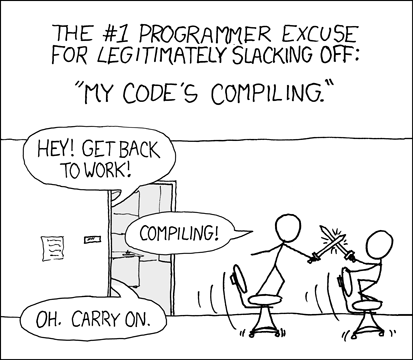
\includegraphics[height=50mm]{images/compiling.png}

<<Компилируется>> \href{https://xkcd.com/303/}{xkcd 303}
\end{center}

Системы сборки (такие как \texttt{make}, \texttt{cmake}, \texttt{autotools}, \texttt{qmake}) позволяют осуществлять инкрементальную сборку, когда компилируется заново только изменившаяся часть кода.


TODO рисунок с примером с и ссылка на рисунок






















\section{Зачем нужна IDE при написании программ? //TODO}

integrated development environment (IDE)
IDE  интегрированная среда разработки

Несколько очевидных пунктов:
подсветка синтаксиса
автодополнение кода
отладчик
автоматическое форматирование кода
интеграцию с системой контроля версий

Использование всего этого в разы повышает эффективность написания кода.


\href{https://www.qt.io/development-tools}{Qt Creator}




















\section{Комментарии в исходном коде}
\epigraph{\textit{Always code as if the guy who ends up maintaining your code will be a violent psychopath who knows where you live.}

\vspace{6pt} % перевод отбивают на 4–8 п

Пишите код так, как будто поддерживать его будет склонный к насилию психопат, который знает, где вы живёте.}{John F. Woods, 1991}

\textit{Комментарии}~-- пояснения к исходному тексту программы, находящиеся непосредственно внутри комментируемого кода.

%Большую часть времени программисты проводят за чтением исходного кода (своего или чужого). Понимание работы программы зависит от структурированности кода и разделению его на модули, выполняющие чётко обозначенные задачи. Для улучшения качества кода или просто оставить заметку прямо внутри кода служат комментарии.

В языке Си \textit{блочным комментарием} является последовательность символов заключённая между \texttt{/*} (началом блочного комментария) и \texttt{*/} (концом). В том числе внутри комментария могут содержаться символы перевода строки, поэтому блочные комментарии также известны как \textit{многострочные}.

\begin{lstlisting}[title=Пример блочного комментария]
int counter = 0;
/*
This is the comment body.
a = a + 42;
*/
counter += a;
\end{lstlisting}

Строки 2-5 содержат блочный комментарий и его содержимое будет проигнорировано компилятором.

Блочный комментарий удобно использовать внутри строки с кодом:
\begin{lstlisting}
void function(int a,/* IN */ int res/* OUT */)
\end{lstlisting}

Следует быть внимательным при использовании блочных комментариев. Попытка вложить один блочный комментарий в другой завершится неудачей, потому что препроцессор удалит текст между \texttt{/*} и первой встретившейся последовательностью символов \texttt{*/}.

\begin{lstlisting}
/*
int var1;
/*
int var2;
*/
int var3;
*/
\end{lstlisting}

Выше приведён пример ошибочного кода. По подсветке синтаксиса можно заметить, что строки 6-7 остались незакомментированными. И компилятор, встретив неизвестные ему символы в 7 строке, выдаст ошибку компиляции:

\begin{small}
\begin{verbatim}
3:1: warning: "/*" within comment [-Wcomment]
7:2: error: expected identifier or ‘(’ before ‘/’ token
\end{verbatim} 
\end{small}

В сообщении компилятора содержится имя файла (не показано), номер строки и позиция символа в строке (\texttt{3:1}~-- третья строка, первый символ), уровень важности (ошибка, предупреждение, заметка) и само сообщение.

К счастью, эта ошибка легко обнаруживается ещё во время написания кода (по подсветке синтаксиса) и компилятором.

Язык Си со стандарта \texttt{C99} поддерживает также \texttt{однострочные комментарии}. Комментарием считается текст после символов \texttt{//} и до окончания строки (до символа перевода строки).

\begin{lstlisting}[title=Пример однострочного комментария]
int counter = 0; //one line comment
a = a + 42;
\end{lstlisting}

В 1 строке содержится однострочный комментарий.

Комментарии часто используются для временного отключения части кода. С этой же целью могут использоваться директивы препроцессора (\texttt{\#if 0 … \#endif}).



\subsection{Принципы написания комментариев}
Комментарии не пишутся, когда:
\begin{itemize}
\item код тривиален и не требует дополнительных пояснений;
\item имена переменных и функций дают достаточно контекста для понимания кода. Например, \texttt{sum\_array} и \texttt{result} -- хорошие имена для переменной, хранящей вычисленную сумму массива, а \texttt{r} и \texttt{sss} -- нет;
\item код пишется для одноразовой задачи, которую нужно выполнить в сжатые сроки.
\end{itemize}

Комментарии пишутся, когда:
\begin{itemize}
\item необходимо пояснить общую суть происходящего в коде.
\item на написание кода было потрачено много времени, чтобы в следующий раз при чтении кода можно было быстрее разобраться (читающему или вам самим), что делает код;
\item необходимо оставить пометку в коде, что часть функционала пока не реализована или содержит проблемы. Для этих целей обычно используется слово \texttt{TODO} в начале комментария, которое распознают многие IDE и редакторы кода;
\item в коде содержатся <<обходные пути>> для особых случаев или <<некрасивые>> решения, которые требуют пояснения, почему было сделано именно так. Пример:
\begin{lstlisting}
// $\color{red}\textrm{на ноль делить нельзя, возвращаем ошибку}$
if (div == 0) return -1;
\end{lstlisting}
\item код реализует известный алгоритм. Например, лучше написать комментарий <<поиск элемента в массиве методом деления отрезка пополам>>, чем комментировать каждую строчку реализации этого алгоритма;
\item всегда.
\end{itemize}

Пример <<плохих>> комментариев:
\begin{lstlisting}
// $\color{red}\textrm{записываем в переменную ноль}$
int i = 0;
// $\color{red}\textrm{обнуляем переменную для результата}$
int result = 0;

// $\color{red}\textrm{цикл пока i меньше или равно 10}$
while (i <= 10) {
    // $\color{red}\textrm{на каждой итерации цикла добавляем к результату}$
    // $\color{red}\textrm{значение переменной i}$
    result = result + i;
    // $\color{red}\textrm{увеличиваем счётчик цикла}$
    i++;
} // $\color{red}\textrm{конец цикла}$
\end{lstlisting}

Несмотря на казалось бы большое количество комментариев, совершенно не очевидно что делает код. Хуже всего то, что комментарии дублируют написанный код и мешают чтению кода.

На начальном этапе обучение языку Си написание таких излишне подробных комментариев допустимо. Однако, не следует излишне подробно описывать тривиальные вещи.

Пример <<хороших>> комментариев для этого же кода:
\begin{lstlisting}
int i = 0;
int result = 0;

// $\color{red}\textrm{считаем сумму чисел от 0 до 10 включительно}$
while (i <= 10) {
    result = result + i;
    i++;
}
\end{lstlisting}

Комментарий полностью описывает происходящее в строках~5-8. Использование имени \texttt{i} для переменной~-- счётчика цикла~-- является общепринятым и в дополнительном пояснении не нуждается (подробнее в for). %TODO). 
Так и имя переменной \texttt{result} является <<говорящим>>.

При написании комментариев стоит помнить о необходимости поддержания актуальности комментариев. Допустим, возникла необходимость внести изменения в код: считать сумму не до 10, а до 20.
\begin{lstlisting}
int i = 0;
int result = 0;

// $\color{red}\textrm{считаем сумму чисел от 0 до 10 включительно}$
while (i <= 20) {
    result = result + i;
    i++;
}
\end{lstlisting}

В код внесли изменения (5~строка), протестировали и убедились, что программа работает правильно. А комментарий изменить забыли (4~строка). Рано или поздно расхождение кода с комментарием обнаружится, и программисту останется только гадать: ошибка в коде или в комментарии?

Хуже отсутствующего комментария может быть только неправильный.





\subsection{Документирование кода}

Ещё одним применением комментариев является аннотирование кода, то есть написание документации прямо внутри комментариев. В дальнейшем эти аннотации извлекаются специальными инструментами для автоматической генерации документации (де-факто \href{http://www.doxygen.nl/}{doxygen} и другие) и создаётся человеко-читабельная документация в формате HTML, PDF и других.

\lstinputlisting[title=Пример написания аннотации к функции \texttt{main}]{examples/doxygen.c}
\noindent
\begin{small}
\begin{tabularx}{\textwidth}{|l|X|}
\hline
\textbf{Строки} & \textbf{Описание}\\
\hline
1 & начало блочного комментария\\
\hline
2 & краткое описание функции в одну строку\\
\hline
3-6 & подробное описание функции. Переносы строк начальные символы игнорируются, в сгенерированном файле описание будет выглядеть так:\newline \texttt{Execution of the program starts here.}\\
\hline
7-8 & описание каждого аргумента функции\\
\hline
9 & описание возвращаемого значения функцией\\
\hline
10 & конец блочного комментария\\
\hline
11-13 & функция \texttt{main}\\
\hline
\end{tabularx}
\end{small}

Пример реальной документации, сгенерированной doxygen, можно посмотреть по ссылке \url{https://libevent.org/doc/} (библиотека libevent).





























% TODO немного объяснить про main и что код пишется там!





\vfill
\subsection*{Контрольные вопросы}
\begin{enumerate}
\item Какое расширение у файлов, содержащих исходный код на языке Си?
\item Перечислите три этапа компиляции программы в исполняемый файл.
\item Чем отличается статическая библиотека от динамической?
\item Как можно отключить часть кода, не удаляя его из файла?
\item Для каких ещё целей могут служить комментарии в исходном коде?
\end{enumerate}
\end{document}
